\section{Implementazione}
In seguito all'analisi e alla formulazione del modello relativo al problema, si è sviluppato uno strumento software basato su un solver per verificare la validità dei concetti prima esposti. Lo strumento software è stato sviluppato in Java e come solver è stato utilizzato Gurobi. In questa sezione si presenterà suddetto strumento e si esporranno le strutture dati utilizzate.
\subsection{Gurobi}
Gurobi Optimizer è un solver commerciale sviluppato da Gurobi Optimization, LLC. Il nome viene dagli autori Dr. Zonghao Gu, Dr. Edward Rothberg e Dr. Robert Bixby, che fondarono Gurobi nel 2008. Gurobi viene utilizzato per problemi di programmazione lineare, programmazione quadratica, programmazione a vincoli quadratici, programmazione lineare mista intera, programmazione quadratica mista intera e programmazione a vincoli quadratici mista intera. Ad oggi, Gurobi viene utilizzato da più di 40 industrie ed è uno dei solver più utilizzati dalle aziende big tech\cite{GUROBIPAGE}.
\subsection{Strutture dati, rappresentazione dell'istanza e dati tecnici}
Si è diviso il progetto in due pacchetti:
\begin{itemize}
	\item model: contiene le classi relative al modello e ai suoi vincoli, assieme ad una classe di util per la configurazione e la classe Main.
	\item data: contiene le classi e le informazioni utili a organizzare i dati necessari per il modello.
\end{itemize}
All'interno di data, è presente una raccolta di istanze divise in BAx.txt e EXx.txt, in base al tipo di problema che si vuole risolvere (base o esteso). Questi file contengono i dati relativi al fabbisogno e ai lavoratori, dei quali si salvano alcuni dati anagrafici, la tipologia contrattuale e le skill che possiede nel caso degli EXx.txt. La classe Worker serve per salvare i dati relativi al cassiere, di cui:
\begin{itemize}
	\item EmploymentType: un enum che contiene le informazioni relative alla tipologia contrattuale, come monte ore settimanale previsto, ore settimanali massime assegnabili e numero massimo di turni giornalieri.
	\item id: un long che rappresenta univocamente il cassiere.
\end{itemize}
Le skill vengono salvate mediante un enum chiamato, sorprendentemente, Skill. La classe Instance si occupa della preparazione dei dati necessari per il modello, come i turni e l'insieme dei lavoratori. All'interno di Instance, viene anche pregenerato l'insieme I11, che contiene le coppie di turni. Le strutture dati principali utilizzate sono:
\begin{itemize}
	\item List: per salvare i turni.
	\item Set: per salvare i lavoratori, separati per tipologia contrattuale.
	\item Map: per  collegare tra loro diversi dati, come il turno agli slot che copre.
\end{itemize}
Per il trasferimento di dati, rispetto a turni o anche successivamente ai lavoratori rispetto ai turni, si utilizzano i Record. I dati vengono letti mediante parsing dai file di testo (questo più avanti verrà ripreso come possibile punto di estensione, introducendo file .json o .xml).

Si passa ora al pacchetto model, il quale è separato nelle seguente classi:
\begin{itemize}
	\item Config: una classe di configurazione, contiene costanti utili per impostare il problema;
	\item Main: esegue il loop di ottimizzazione sulle istanze generate e richiama i metodi necessari per stampare i risultati;
	\item PersonnelSchedulingBaseModel e ExtendedModel: il cuore dell'intero progetto, in quanto contengono tutti i vincoli relativi al modello;
	\item SolutionPrinter: stampa le soluzioni su un file di .csv. estendere questo?
\end{itemize}
All'interno di PersonnelSchedulingBaseModel, tramite la programmazione lineare si rappresentano i vincoli; si riporta un esempio di codice che rimanda ai vincoli di massimo numero di turni assegnabili per giorno:
\begin{lstlisting}[caption={Esempio di metodo per i vincoli}, style=java, label={lst:esempio_java}]
public void maxTurnsPerDay() throws GRBException {
	for (Worker w : instance.getAllWorkers()) {
		for (int day = 1; day <= Instance.TIMEWINDOW; day++) {
			
			int maxT = w.getType().maxTurns(day);   
			GRBLinExpr lhs = new GRBLinExpr();
			
			for (Shift s : instance.getDayByShifts(day)) {
				GRBVar xcs = x_CS_Var.get(new WorkerShift(w.getId(), s.id()));
				if (xcs != null) lhs.addTerm(1.0, xcs);
			}
			
			model.addConstr(lhs, GRB.LESS_EQUAL, maxT,
			"MaxTurns_w" + w.getId() + "_d" + day);
		}
	}
}
\end{lstlisting}
Le strutture dati utilizzate sono le stesse utilizzate per Instance, con la differenza che in queste due classi le Map assumono un ruolo più fondamentale, in quanto stanno alla base dell'intera costruzione del modello collegando le variabili di Gurobi ai relativi dati. Le Map utilizzate sono le seguenti:
\begin{lstlisting}[caption={Map usate per le variabili del modello}, style=java, label={lst:structureMap}]
private final Map<DaySlot, GRBVar> u_DK = new HashMap<>();
private final Map<WorkerShift, GRBVar> x_CS_Var = new HashMap<>();
private final Map<WorkerDay, GRBVar> splitC_D = new HashMap<>();
private final Map<WorkerDay, GRBVar> staccoC_D = new HashMap<>(); 
private final Map<WorkerDay, GRBVar> riposoC_D = new HashMap<>();
\end{lstlisting}
\textit{DaySlot}, \textit{WorkerShift} e \textit{WorkerDay} sono dei Record. Si utilizzano le seguenti classi di Gurobi per implementare il modello:
\begin{itemize}
	\item GRBEnv: l'environment per Gurobi, fondamentale per impostare tutto.
	\item GRBModel: l'oggetto che rappresenta il modello per Gurobi. I metodi utilizzati per questa classe sono: addVar e addConstr per aggiungere variabili e vincoli, setObjective per impostare l'obiettivo, optimize per ottimizzarlo.
	\item GRBVar: le variabili del modello per Gurobi, aggiunte mediante addVar al modello.
	\item GRBLinExpr: un'espressione lineare, importante per la definizione dei vincoli.
\end{itemize}
Le funzioni obiettivo sono salvate mediante GRBLinExpr. Per la funzione obiettivo si sono trovate due strade:
\begin{itemize}
	\item Metodo pesato: come espresso nella sezione 3, si sommano tutti gli obiettivi assegnandogli i specifici pesi e si esegue poi l'ottimizzazione del modello.
	\item Metodo gerarchico: si dà una priorità agli obiettivi, si ottimizza prima rispetto all'obiettivo con priorità più alta, si passa poi a quelli con priorità più bassa aggiungendo un vincolo che garantisca il non peggioramento dell'obiettivo precedente. 
\end{itemize}
In Gurobi, per entrambi gli approcci si può adoperare il seguente metodo:
\begin{lstlisting}[style=java, label={lst:setObjective}]
void setObjectiveN(GRBLinExpr expr, int index, int priority, double weight, double abstol, double reltol, String name)
\end{lstlisting}
ove:
\begin{itemize}
	\item expr: obiettivo.
	\item index: indice dell'obiettivo, utile per il log.
	\item priority: priorità all'interno della gerarchia di ottimizzazione.
	\item weight: peso assegnato all'obiettivo.
	\item abstol: tolleranza assoluta per l'obiettivo, ovvero di quanto può degradare la soluzione quando si ottimizzano obiettivi secondari (stessa unità dell'obiettivo).
	\item reltol: tolleranza relativa per l'obiettivo, come abstol ma relativo (percentuale dell'obiettivo).
	\item name: nome dell'obiettivo, utile per il log.
\end{itemize}
Per esprimere correttamente quanto esposto nella sezione 3, il metodo è stato usato con la priorità imposta uguale per tutti gli obiettivi, tuttavia si potrebbe comunque risolvere il problema dando priorità maggiore alla copertura e a eventuali obiettivi di equità e minimizzazione delle ore, così da garantire una soluzione migliore per gli obiettivi principali.

Si introduce infine la classe SolutionPrinter. Questa classe contiene metodi utili alla stampa della soluzione trovata da Gurobi, in particolare risultano fondamentali:
\begin{itemize}
	\item writeSolutionCsvTablesByWorker: salva su un file .csv gli orari separati per singolo cassiere.
	\item exportUtoCsv: salva su un file .csv una tabella contenente i valori di $u(d,k)$ per ogni slot temporale, mostrando come si comporta Gurobi.
	\item writeObjectiveResult: ritorna un file .txt con i valori trovati per singolo obiettivo.
\end{itemize}
Si riporta un esempio di tabella oraria generata da writeSolutionCsvTablesByWorker:
\begin{center}
	\includegraphics[width=75mm]{figures/esempioorario.png}
\end{center}
\pagebreak
\subsection{Risultati implementativi}
In quanto disponibili, gli esperimenti sono stati eseguiti su una macchina con le seguenti specifiche tecniche:
\begin{itemize}
	\item AMD Ryzen™ 7 5700X CPU @ 3.40GHz × 16.
	\item 32GB RAM 3200MHz.
\end{itemize}
I test sono stati eseguiti su 3 istanze per il modello base e 3 istanze per il modello esteso, dando 3 diversi limiti di tempo (5, 10 e 30 minuti). I valori dei pesi sono riportati nell'appendice, mentre per i relativi significati dietro i valori dei singoli obiettivi si rimanda alla sezione 3.

Le versioni di Java e Gurobi utilizzate sono rispettivamente Java-21 e Gurobi 13.0.0. Si riportano ora i risultati ottenuti con il primo insieme di coefficienti:
\begin{center}
	\begin{tabular}{ c c c c }
		BA1(1) & & Valore ottimo & \\
		\hline
		Tempo limite & 300 & 600 & 1800\\
		\hline
		Valore f.o & 3171.5 & 2985.0 & 1271.5\\
		Gap(\%) & 62.6 & 60.3 & 6.76\\
		\hline
		$f_1$ & 1980.0 & 1800.0 & 40.0\\
		$f_2$ & 1098.5 & 1110.0 & 1150.5\\
		$f_3$ & 93.0 & 75.0 & 81.0\\
		\hline
	\end{tabular}
\end{center}
\begin{center}
	\begin{tabular}{ c c c c }
		BA2(1) & & Valore ottimo & 8608.0\\
		\hline
		Tempo limite & 300 & 600 & 1800\\
		\hline
		Valore f.o & 8624.0 & 8624.0 & 8624.0\\
		Gap(\%) & 0.19 & 0.19 & 0.19\\
		\hline
		$f_1$ & 8080.0 & 8080.0 & 8080.0\\
		$f_2$ & 516.0 & 516.0 & 516.0\\
		$f_3$ & 28.0 & 28.0 & 28.0\\
		\hline
	\end{tabular}
\end{center}
\begin{center}
	\begin{tabular}{ c c c c }
		BA3(1) & & Valore ottimo & 5206.0\\
		\hline
		Tempo limite & 300 & 600 & 1800\\
		\hline
		Valore f.o & 5242.0 & 5240.0 & 5235.0\\
		Gap(\%) & 0.69 & 0.65 & 0.55\\
		\hline
		$f_1$ & 4340.0 & 4340.0 & 4340.0\\
		$f_2$ & 846.0 & 846.0 & 846.0\\
		$f_3$ & 56.0 & 54.0 & 49.0\\
		\hline
	\end{tabular}
\end{center}
\begin{center}
	\begin{tabular}{ c c c c }
		EX1(1) & & Valore ottimo & 473.0\\
		\hline
		Tempo limite & 300 & 600 & 1800\\
		\hline
		Valore f.o & 474.0 & 473.5 & 473.5 \\
		Gap(\%) & 0.21 & 0.11 & 0.11\\
		\hline
		$f_1$ & 0.0 & 0.0 & 0.0\\
		$f_2$ & 336.0 & 336.0 & 336.0\\
		$f_3$ & 24.0 & 24.0 & 24.0\\
		$f_4$ & 0.0 & 0.0 & 0.0\\
		$f_5$ & 0.0 & 0.0 & 0.0\\
		$f_6$ & 0.0 & 0.0 & 0.0\\
		$f_7$ & -2.0 & -2.0 & -2.0\\
		$f_8$ & 0.0 & 0.0 & 0.0\\
		$f_9$ & 116.0 & 115.5 & 115.5\\
		\hline
	\end{tabular}
\end{center}
\begin{center}
	\begin{tabular}{ c c c c }
		EX2(1) & & Valore ottimo & 10271.0\\
		\hline
		Tempo limite & 300 & 600 & 1800\\
		\hline
		Valore f.o & 10272.5 & 10272.5 & 10272.5\\
		Gap(\%) & 0.01 & 0.01 & 0.01\\
		\hline
		$f_1$ & 8220.0 & 8220.0 & 8220.0\\
		$f_2$ & 516.0 & 516.0 & 516.0\\
		$f_3$ & 36.0 & 36.0 & 36.0\\
		$f_4$ & 92.0 & 92.0 & 92.0\\
		$f_5$ & 0.0 & 0.0 & 0.0\\
		$f_6$ & 180.0 & 180.0 & 180.0\\
		$f_7$ & -4.5 & -4.5 & -4.5\\
		$f_8$ & 0.0 & 0.0 & 0.0\\
		$f_9$ & 1233.0 & 1233.0 & 1233.0\\
		\hline
	\end{tabular}
\end{center}
\begin{center}
	\begin{tabular}{ c c c c } 
		EX3(1) & & Valore ottimo & 1419.3\\
		\hline
		Tempo limite & 300 & 600 & 1800\\
		\hline
		Valore f.o & 1819.7 & 1693.9 & 1669.3\\
		Gap(\%) & 22.0 & 16.2 & 15.0\\
		\hline
		$f_1$ & 120.0 & 0.0 & 0.0\\
		$f_2$ & 1181.0 & 1194.5 & 1187.5\\
		$f_3$ & 218.0 & 208.0 & 205.0\\
		$f_4$ & 89.0 & 102.5 & 95.5\\
		$f_5$ & 21.2 & 14.4 & 10.8\\
		$f_6$ & 143.0 & 135.0 & 138.0\\
		$f_7$ & -5.5 & -5.5 & -5.5\\
		$f_8$ & 0.0 & 0.0 & 0.0\\
		$f_9$ & 53.0& 45.0 & 38.0\\
		\hline
	\end{tabular}
\end{center}
Si riportano ora i risultati ottenuti con il secondo insieme di coefficienti:\\
\begin{center}
	\begin{tabular}{ c c c c }
		BA1(2) & & Valore ottimo & 1165.5\\
		\hline
		Tempo limite & 300 & 600 & 1800\\
		\hline
		Valore f.o & 2280.5 & 2236.5 & 2144.0\\
		Gap(\%) & 48.9 & 47.9 & 45.6 \\
		\hline
		$f_1$ & 990.0 & 990.0 & 900.0\\
		$f_2$ & 1108.5 & 1102.5 & 1106.0\\
		$f_3$ & 182.0 & 144.0 & 138.0 \\
		\hline
	\end{tabular}
\end{center}
\begin{center}
	\begin{tabular}{ c c c c }
		BA2(2) & & Valore ottimo & 4580.0\\
		\hline
		Tempo limite & 300 & 600 & 1800\\
		\hline
		Valore f.o & 4612.0 & 4612.0 & 4612.0\\
		Gap(\%) & 0.69 & 0.69 & 0.69\\
		\hline
		$f_1$ & 4040.0 & 4040.0 & 4040.0 \\
		$f_2$ & 516.0 & 516.0 & 516.0\\
		$f_3$ & 56.0 & 56.0 & 56.0 \\
		\hline
	\end{tabular}
\end{center}
\begin{center}
	\begin{tabular}{ c c c c }
		BA3(2) & & Valore ottimo & 3056.0\\
		\hline
		Tempo limite & 300 & 600 & 1800\\
		\hline
		Valore f.o & 3122.0 & 3118.0 & 3112.0\\
		Gap(\%) & 2.11 & 1.99 & 1.80\\
		\hline
		$f_1$ & 2170.0 & 2170.0 & 2170.0 \\
		$f_2$ & 846.0 & 846.0 & 846.0 \\
		$f_3$ & 106.0 & 102.0 & 96.0 \\
		\hline
	\end{tabular}
\end{center}
\begin{center}
	\begin{tabular}{ c c c c }
		EX1(2) & & Valore ottimo & 470.9\\
		\hline
		Tempo limite & 300 & 600 & 1800\\
		\hline
		Valore f.o & 489.5 & 488.5 & 488.5 \\
		Gap(\%) & 3.8 & 3.6 & 3.6\\
		\hline
		$f_1$ & 0.0 & 0.0 & 0.0\\
		$f_2$ & 336.0 & 336.0 & 336.0\\
		$f_3$ & 50.0 & 52.0 & 24.0\\
		$f_4$ & 0.0 & 0.0 & 0.0\\
		$f_5$ & 0.0 & 0.0 & 0.0\\
		$f_6$ & 0.0 & 0.0 & 0.0\\
		$f_7$ & -10.0 & -10.0 & -10.0\\
		$f_8$ & -3.0 & -6.0 & -6.0\\
		$f_9$ & 116.5 & 116.5 & 116.5\\
		\hline
	\end{tabular}
\end{center}
\begin{center}
	\begin{tabular}{ c c c c }
		EX2(2) & & Valore ottimo & 5854.5\\
		\hline
		Tempo limite & 300 & 600 & 1800\\
		\hline
		Valore f.o & 5866.0 & 5866.0 & 5866.0\\
		Gap(\%) & 0.20 & 0.20 & 0.20\\
		\hline
		$f_1$ & 4110.0 & 4110.0 & 4110.0\\
		$f_2$ & 516.0 & 516.0 & 516.0\\
		$f_3$ & 72.0 & 72.0 & 72.0\\
		$f_4$ & 184.0 & 184.0 & 184.0\\
		$f_5$ & 0.0 & 0.0 & 0.0\\
		$f_6$ & 180.0 & 180.0 & 180.0\\
		$f_7$ & -18.0 & -18.0 & -18.0\\
		$f_8$ & 0.0 & 0.0 & 0.0\\
		$f_9$ & 822.0 & 822.0 & 822.0\\
		\hline
	\end{tabular}
\end{center}
\begin{center}
	\begin{tabular}{ c c c c } 
		EX3(2) & & Valore ottimo & 1419.3\\
		\hline
		Tempo limite & 300 & 600 & 1800\\
		\hline
		Valore f.o & 2528.2 & 2148.9 & 2044.1\\
		Gap(\%) & 41.2 & 30.6 & 27.1\\
		\hline
		$f_1$ & 460.0 & 120.0 & 120.0\\
		$f_2$ & 1150.5 & 1169.5 & 1163.5\\
		$f_3$ & 494.0 & 454.0 & 392.0\\
		$f_4$ & 117.0 & 155.0 & 143.0\\
		$f_5$ & 26.2 & 58.4 & 5.6\\
		$f_6$ & 191.0 & 168.0 & 202.0\\
		$f_7$ & -26.0 & -26.0 & -26.0\\
		$f_8$ & 0.0 & 0.0 & 0.0\\
		$f_9$ & 115.5 & 50.0 & 44.0\\
		\hline
	\end{tabular}
\end{center}
Infine, si riportano gli ultimi dati ottenuti con l'ultimo insieme di coefficienti:
\begin{center}
	\begin{tabular}{ c c c c }
		BA1(3) & & Valore ottimo & 576.9\\
		\hline
		Tempo limite & 300 & 600 & 1800\\
		\hline
		Valore f.o & 916.8 & 886.3 & 857.0\\
		Gap(\%) & 37.1 & 34.9 & 32.7\\
		\hline
		$f_1$ & 202.0 & 198.0 & 164.0\\
		$f_2$ & 558.8 & 552.3 & 555.0\\
		$f_3$ & 156.0 & 136.0 & 138.0\\
		\hline
	\end{tabular}
\end{center}
\begin{center}
	\begin{tabular}{ c c c c }
		BA2(3) & & Valore ottimo & 1090.0\\
		\hline
		Tempo limite & 300 & 600 & 1800\\
		\hline
		Valore f.o & 1122.0 & 1122.0 & 1122.0\\
		Gap(\%) & 2.85 & 2.85 & 2.85\\
		\hline
		$f_1$ & 808.0 & 808.0 & 808.0\\
		$f_2$ & 258.0 & 258.0 & 258.0\\
		$f_3$ & 56.0 & 56.0 & 56.0\\
		\hline
	\end{tabular}
\end{center}
\begin{center}
	\begin{tabular}{ c c c c }
		BA3(3) & & Valore ottimo & 897.0\\
		\hline
		Tempo limite & 300 & 600 & 1800\\
		\hline
		Valore f.o & 968.8 & 954.8 & 954.8\\
		Gap(\%) & 7.41 & 6.05 & 6.05\\
		\hline
		$f_1$ & 454.0 & 436.0 & 436.0 \\
		$f_2$ & 420.8 & 422.8 & 422.8 \\
		$f_3$ & 94.0 & 96.0 & 96.0 \\
		\hline
	\end{tabular}
\end{center}
\begin{center}
	\begin{tabular}{ c c c c }
		EX1(3) & & Valore ottimo & 265.0\\
		\hline
		Tempo limite & 300 & 600 & 1800\\
		\hline
		Valore f.o & 299.0 & 283.0 & 282.5\\
		Gap(\%) & 11.4 & 6.36 & 6.17\\
		\hline
		$f_1$ & 0.0 & 0.0 & 0.0\\
		$f_2$ & 168.0 & 168.0 & 168.0\\
		$f_3$ & 52.0 & 56.0 & 56.0\\
		$f_4$ & 0.0 & 0.0 & 0.0\\
		$f_5$ & 0.0 & 0.0 & 0.0\\
		$f_6$ & 0.0 & 0.0 & 0.0\\
		$f_7$ & -20.0 & -20.0 & -20.0\\
		$f_8$ & -20.0 & -40.0 & -40.0\\
		$f_9$ & 119.0 & 119.0 & 118.5\\
		\hline
	\end{tabular}
\end{center}
\begin{center}
	\begin{tabular}{ c c c c }
		EX2(3) & & Valore ottimo & 1915.3\\
		\hline
		Tempo limite & 300 & 600 & 1800\\
		\hline
		Valore f.o & 1917.0 & 1917.0 & 1917.0\\
		Gap(\%) & 0.09 & 0.09 & 0.09\\
		\hline
		$f_1$ & 1062.0 & 1062.0 & 1062.0 \\
		$f_2$ & 228.0 & 228.0 & 228.0 \\
		$f_3$ & 72.0 & 72.0 & 72.0\\
		$f_4$ & 64.0 & 64.0 & 64.0\\
		$f_5$ & 0.0 & 0.0 & 0.0\\
		$f_6$ & 0.0 & 0.0 & 0.0\\
		$f_7$ & -40.0 & -40.0 & -40.0\\
		$f_8$ & 0.0 & 0.0 & 0.0\\
		$f_9$ & 531.0 & 531.0 & 531.0\\
		\hline
	\end{tabular}
\end{center}
\begin{center}
	\begin{tabular}{ c c c c }
		EX3(3) & & Valore ottimo & 999.4\\
		\hline
		Tempo limite & 300 & 600 & 1800\\
		\hline
		Valore f.o & 1232.5 & 1228.5 & 1222.5\\
		Gap(\%) & 18.9 & 18.6 & 18.2\\
		\hline
		$f_1$ & 306.0 & 306.0 & 306.0\\
		$f_2$ & 546.0 & 546.0 & 546.0\\
		$f_3$ & 304.0 & 290.0 & 284.0\\
		$f_4$ & 0.0 & 0.0 & 0.0\\
		$f_5$ & 0.0 & 0.0 & 0.0\\
		$f_6$ & 0.0 & 0.0 & 0.0\\
		$f_7$ & -56.0 & -56.0 & -56.0\\
		$f_8$ & -40.0 & -30.0 & -30.0\\
		$f_9$ & 172.5 & 172.5 & 172.5\\
		\hline
	\end{tabular}
\end{center}
\pagebreak
Si mostrano ora dei grafici che mostrano il miglioramento della soluzione trovata da Gurobi rispetto al tempo.
\begin{center}
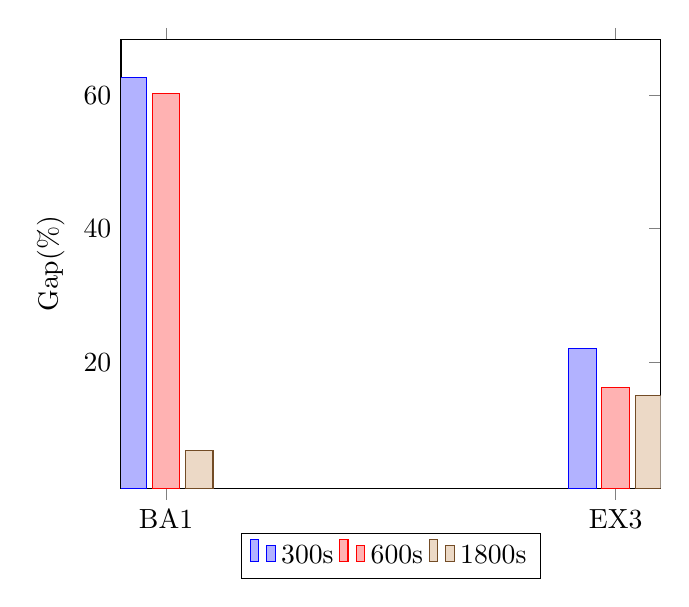
\begin{tikzpicture}
	\begin{axis}[
		ylabel=Gap(\%),
		symbolic x coords={BA1,EX3},
		xtick=data,
		legend style={at={(0.5,-0.1)}, anchor=north, legend columns=-1},
		ybar,
		]
		\addplot coordinates {(BA1, 62.7) (EX3, 22.0)};
		\addplot coordinates {(BA1, 60.3) (EX3, 16.2)};
		\addplot coordinates {(BA1, 6.76) (EX3, 15.0)};
		\legend{300s,600s,1800s}
	\end{axis}
\end{tikzpicture}\\
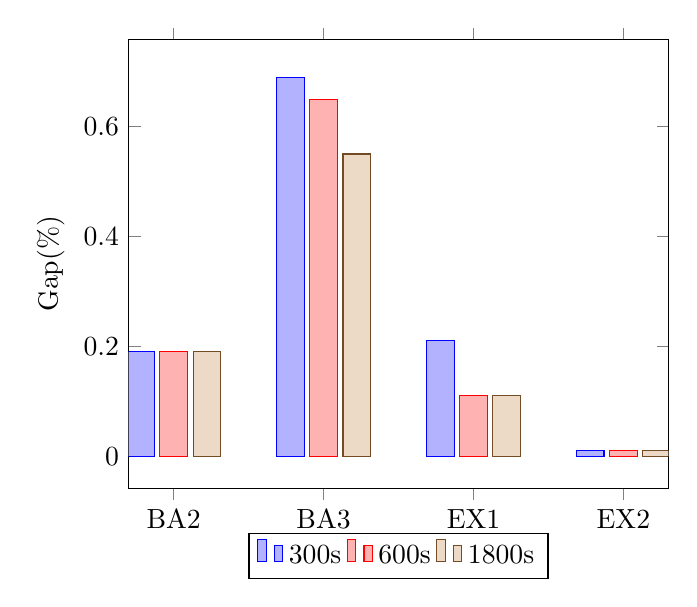
\begin{tikzpicture}
	\begin{axis}[
		ylabel=Gap(\%),
		symbolic x coords={BA2,BA3,EX1,EX2},
		xtick=data,
		legend style={at={(0.5,-0.1)}, anchor=north, legend columns=-1},
		ybar,
		]
		\addplot coordinates {(BA2, 0.19) (BA3, 0.69) (EX1, 0.21) (EX2, 0.01)};
		\addplot coordinates {(BA2, 0.19) (BA3, 0.65) (EX1, 0.11) (EX2, 0.01)};
		\addplot coordinates {(BA2, 0.19) (BA3, 0.55) (EX1, 0.11) (EX2, 0.01)};
		\legend{300s,600s,1800s}
	\end{axis}
\end{tikzpicture}
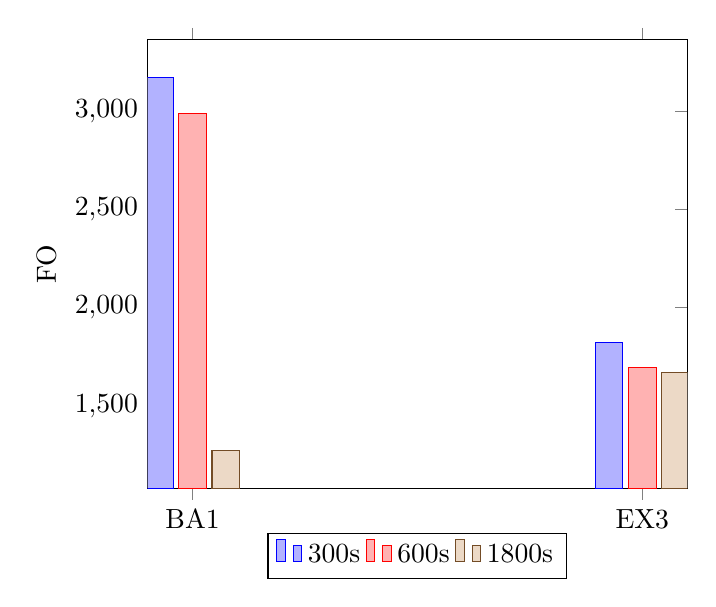
\begin{tikzpicture}
	\begin{axis}[
		ylabel=FO,
		symbolic x coords={BA1,EX3},
		xtick=data,
		legend style={at={(0.5,-0.1)}, anchor=north, legend columns=-1},
		ybar,
		]
		\addplot coordinates {(BA1, 3171.5) (EX3, 1819.7)};
		\addplot coordinates {(BA1, 2985.0) (EX3, 1693.9)};
		\addplot coordinates {(BA1, 1271.5) (EX3, 1669.3)};
		\legend{300s,600s,1800s}
	\end{axis}
\end{tikzpicture}
\end{center}
Questi risultati sono stati ottenuti eseguendo l'istanza una singola volta con il limite di tempo dato. Non sono stati impostati dei vincoli relativi a numero di thread o valori per il seed. Per quasi tutte le soluzioni, Gurobi segna uno stato per la soluzione pari a TIME\_LIMIT, in quanto, per via della natura del problema, trovare la soluzione ottima risulta complesso. Lo stato viene segnato come OPTIMAL per le soluzioni delle istanze EX1 e EX2 con un limite di tempo di 30 minuti. Sia per EX1 che per EX2, si nota però che Gurobi ha trovato una soluzione identica anche con altri limiti di tempo. Per l'istanza EX2 con tempo limite pari a 10 minuti, si nota che l'ultimo best bound trovato è di 10254.1 e non 10271.0 come riportato nella tabella: il best bound viene ottenuto mediante rilassamento e viene migliorato nel tempo grazie a varie tecniche, come cutting planes (es. Gomory), branch and bound, pruning o presolve. I valori ottimi inseriti nelle varie tabelle rappresentano il best bound trovato nei test sulle istanze con limite di tempo pari a 30 minuti e il gap individuato per ogni soluzione è stato ricalcolato sulla base di questo: se si osservano i log, per esempio si può osservare come il gap per la soluzione trovata per EX2 con tempo limite pari a 10 minuti sia uguale allo 0.18\%, in quanto calcolato rispetto al best bound citato prima di 10254.1.